% !TEX encoding = UTF-8 Unicode
\chapter{Literature review, objectives, and contribution} \label{chap-lit-review}

The literature review was in two parts. The first part, which is summarised in Section \ref{sec:lit-grinding}, describes previous research related to grinding process control. This includes an introduction to the dynamics of the grinding process and work on grinding process control, process observers, and grinding process disturbances. Section \ref{sec:objectives} relates the main observations from the literature to the objectives of the thesis. The second part of the literature review, presented in Section \ref{sec:lit-disturb-models}, introduces the methods proposed to tackle the research problem: industrial process disturbance models, observers for estimating disturbances, and other relevant methods. Section \ref{sec:contributions} lists the main contributions of this research.

\section{Literature review part 1 – grinding process control} \label{sec:lit-grinding}

\subsection{The grinding process}

Figure \ref{fig:cause-effect} is a schematic diagram illustrating the main cause-effect relationships in a tumbling mill. Each oval represents an important process variable and the arrows represent the interacting relationships and the direction of causality. The five variables on the left are the main input variables and the four on the right are the main outputs or measurements. Mill contents and breakage rates are internal variables of the process. Here, mill contents has a broad definition encompassing all attributes of the contents, including water, slurry, ore particles, and grinding media.
\begin{figure}[htp]
	\centering
	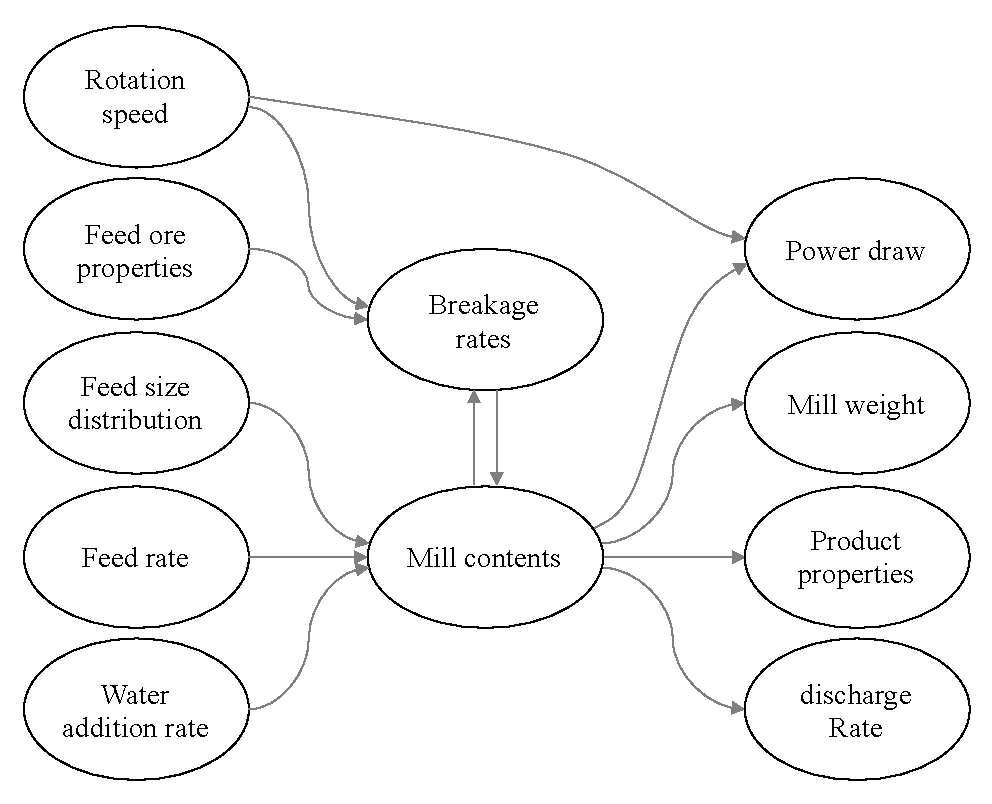
\includegraphics[width=11cm]{images/cause-effect.pdf}
	\caption{Cause and effect diagram} \label{fig:cause-effect}
\end{figure}

\cite{powell_applying_2009} highlighted the interactive (i.e. bi-directional) relationship between mill contents and breakage rates and describe how these variables evolve dynamically. A change in ore feed properties, such as a change in hardness or particle sizes, leads to changes in the mill contents, which then affect breakage rates, which have a feedback effect on the evolution of the mill contents. This results in a non-linear response of the output variables that depends on the mill contents.

As mentioned in the introduction, changes in ore feed properties have a significant impact on the process. \cite{morrell_influence_2001} stated that variations in ore competency and the feed size distribution are the top two factors having the greatest influence on \acrshort{SAG} mill performance.

\acrshort{SAG} mills are usually installed in closed-circuit with a pump and a classifier, as in the example shown in Figure \ref{fig:sag-ball-circuit-diag}. Oversize material that passed through the discharge grate of the mill but does not meet the specification of the classifier is returned to the mill, sometimes via a crusher. This feedback mechanism has a transport delay, which further complicates the dynamic response of the process variables to changes in the inputs.

\subsection{Grinding process control}

The objectives of process control in grinding applications are firstly, to maintain a steady operation and secondly, to optimize the process conditions to maximize operational benefits, for example, maximizing throughput while meeting the product particle size specification \citep{wei_grinding_2009}. Inevitably, trade-offs must be made between competing output objectives, such as throughput and product particle size, and between product particle size and power consumption. The focus of this work is to identify and develop methods that facilitate the first objective (i.e. steady operation) given a set of desired operating conditions.

According to a 2007 worldwide survey of grinding circuit operators \citep{wei_grinding_2009}, 63\% reported that \gls{PID} control was used. \textit{Multivariable control} or \textit{expert systems} were used by 21\%. Less than 10\% reported using \gls{MPC} or adaptive (self-tuning) control.

The three most commonly controlled variables are the product particle size, the slurry level in the sump, and the sump discharge slurry density. The mill load or filling level also requires some form of control since excursions above or below the normal range can lead to undesirable conditions such as \textit{mill overload} and \textit{freewheeling} \citep{mcclure_overload_2015}. If the load becomes too high, the mill may have to be stopped, resulting in lost production \citep{wei_grinding_2009}.

The main manipulated variables used for control are the set points of the water flow rate to the sump, the water flow rate to the mill, the feed rate of solids to the mill, and the slurry discharge flow rate from the sump. Many modern mills also have variable speed drives which allow controlled variation of the rotational speed. However, use of speed as a manipulated variable was reported by less than 10\% of respondents in \cite{wei_grinding_2009}.

There is an extensive academic literature on the application of process control theory and methods to grinding, going back as far as the 1980s, e.g. \cite{herbst_optimal_1988}. A wide variety of techniques have been proposed and evaluated since then. Most of the results are based on computer simulations of control systems applied to simulation models of grinding processes. In many cases, these simulations include ore disturbances.

\cite{najim_adaptive_1995} simulated various adaptive controllers applied to a grinding circuit model with a step disturbance in the ore hardness, represented by a 20\% reduction in breakage rates. In their work, the controllers regulate the circulating load and product size by manipulating the water addition rate and the fresh ore feed rate.

\cite{pomerleau_survey_2000} simulated various control algorithms applied to a grinding process consisting of a rod mill and a ball mill. The controllers manipulated the set points of the fresh ore and the water feed rate to regulate the product fineness and the circulating load. To compare the performance of the controllers, they simulated a sequence of disturbances to two ore properties---\textit{grindability} and feed size---as well as a change in the number of active cyclones and set point changes to controlled variables.

\cite{chen_disturbance_2009} proposed a \gls{DOB} control strategy applied to a ball mill grinding circuit model and evaluated its effectiveness in suppressing the effects of a 10\% increase in ore hardness on the product fineness and circulating load.

\cite{estrada_hybrid_2014} simulated a \gls{HNMPC} system to minimize specific energy consumption while regulating the product particle size. Hybrid approaches allow discrete variables to be included in the plant model. These are useful for representing processes which have discrete operating modes, such as those with equipment items that may be switched on or off during operation. They used this to represent changes in the stockpile feeding process and the activation of secondary grinding circuits. They presented simulation results showing how the controlled system responded as the different ore feed streams were switched off and on.

\cite{le_roux_throughput_2016} simulated a non-linear model-based control architecture to independently control the throughput and product quality of a grinding circuit. To achieve this, they used the set points for mill speed, feed rate, water addition, and cyclone feed rate as manipulated variables. \cite{botha_hybrid_2018} simulated a \gls{HNMPC} system for a primary grinding mill circuit in which the number of hydrocyclones (a discrete variable) is used as an additional manipulated variable. The switching of hydrocyclones has a large dynamic influence on the plant. They show that this increased controller stability compared to nonlinear \gls{MPC} without this discrete variable.

\cite{aguila-camacho_control_2017} simulated various types of \textit{fractional order controllers} applied to a grinding circuit model with five manipulated input variables (fresh ore feed rate, mill inlet feed water rate, sump feed water rate, cyclone feed flow rate, and ball addition rate) and three output variables (mill filling level, sump slurry volume, and product fineness). They also simulated step changes in the ore feed size distribution and in energy required to break ore particles, which is similar to ore hardness.

There is less literature available on the implementation, performance, and benefits of control systems in actual operations. \cite{herbst_optimal_1988} presented results of implementing an optimal control algorithm (\gls{LQG}) on a rod and ball mill grinding circuit in North America. This included use of an extended Kalman filter to estimate the states and parameters of a non-linear phenomenological model. The results show that the observer estimates tracked the process output measurements in response to a change in ore hardness, and the corresponding changes in model parameters.

\cite{hulbert_multivariable_1990} presented results of implementing a multi-variable controller on an AG mill in South Africa. The manipulated variables were the set points for the ore feed rate to the mill, the water feed rate to the sump, and the flow rate of slurry to the cyclone. The controlled variables were product particle size, mill load, and slurry level in the sump. They show the responses of the controlled system to set point changes and state that implementation of the multivariable controller resulted in better control of the product size and an increase in throughput.

\cite{desbiens_distributed_1997} described the development and implementation of a \gls{PI} regulatory control strategy on a grinding circuit at a mine in Ontario, including the steps of process model identification and filter design. The installed system regulates the pump box level, the cyclone feed density and the cyclone overflow density by manipulating the pump box water addition set point, the rod mill water addition set point, and the rod mill ore feed rate set point.

One of the case studies presented by \cite{desbiens_using_2008} described the implementation of an improved grinding circuit control strategy in a copper concentrator in Peru. They addressed the problem of quickly adjusting the rod-mill feed rate when a change in ore hardness occurred. This was achieved by simultaneously manipulating the rod mill feed rate and a flow splitter controlling the flows to the ball mills according to the levels in the pump boxes. After implementation of the new control system, the variability in process conditions reduced, the average throughput increased by 4\%, and the combined circuit energy consumption reduced by 8 to 10\%.

\cite{nunez_self-optimizing_2009} described the development and implementation of regulatory controls at a mine in Canada. The grinding process consisted of two parallel circuits, each containing an open-circuit rod mill and a ball mill in closed-circuit. They reported that ore hardness changes were leading to either over or under-grinding and mill overload situations, which were not always detected in time by the operators. The new system consisted of two distributed control loops on each circuit, one to control the pump-box level by manipulating the rod mill feed set point, and the second to control the cyclone overflow density (in the absence of a product particle size analyser) by manipulating the pump box water addition rate set point. The results indicated a significant (60\%) reduction in variability of the product density and a 7.7\% increase in throughput for the same level of energy consumption, no change to mineral recovery, and the avoidance of mill overloads.

\cite{yutronic_sag_2011} described the development and implementation of an \gls{MPC}-based control strategy at a large concentrator plant in Chile. The primary goal was to reduce process variability in the \acrshort{SAG} circuits, and in particular, the effects of poor sump level control on classification efficiency. The \acrshort{SAG} filling level was deemed to be the most important process variable, due to its relationship with grinding efficiency. Since filling level is not measurable, the mill weight was used as the controlled variable, along with the power draw, the shell impact noise level, the motor torque, and the produced pebble flow rate. The \gls{MPC} included constraints on certain process variables, such as the power draw to avoid electrical overload. The manipulated variables were the fresh ore feed rate set point, mill speed set point and the solids-to-water ratio of the feed. Two measured disturbances were also included in the \gls{MPC} model, the returned pebble flow rate and the fine ore percentage in the feed. As a result of implementing the \gls{MPC} system, the variability of the cyclone feed solids content and feed pressure were reduced by 43\% and 22\%, respectively. Other benefits included higher throughput, lower specific energy consumption, and a 4.8\% reduction in the average \acrshort{SAG} product size.

\cite{steyn_benefits_2013} presented results of implementing \gls{MPC} on an \gls{AG} mill in South Africa with the goal of reducing variability and to ``continuously drive towards the optimal operating point within system constraints.'' The two main controlled variables were power consumption and mill load. They report a 66\% reduction in power and a 40\% reduction in the standard deviation of the mill load as a result of implementing the \gls{MPC}. This reduction in process variability also enabled steady-state experiments to be conducted to determine the optimal product particle size for a given mill feed rate, which led to a subsequent improvement in mineral recovery.

\cite{gough_sag_2015} reported using \gls{MPC} to control the mill weight, feed rate, and rotation speed of various \acrshort{SAG} mills at mines in South America. The controller included measured disturbances such as pebble recycle rate and ore size distribution as feed forward inputs to improve control. He presented results showing that the \gls{MPC} is able to reduce the variability in mill weight (84\% reduction in standard deviation) and throughput (55\% reduction in standard deviation) compared to the expert systems that were used in these facilities, resulting in increased production.

\cite{bouchard_reducing_2017} showed how a properly designed control system can enable higher utilization of grinding circuit capacity and a reduction in specific energy consumption (\acrshort{kWh}/ton). They used a simulation model of a rod and ball mill circuit to compare three different control strategies. Firstly, a basic \gls{PI} regulatory strategy to control the pump box level by manipulating the water addition set point to the pump box and to control the hydrocyclone pressure by manipulating the cyclone feed rate set point. Secondly, a \gls{PI} regulatory strategy to control the pump box level by manipulating the rod mill feed rate set point, and the product particle size (\acrshort{P80}) by manipulating the water addition set point to the pump box. Thirdly, an \gls{MPC} (multivariable) strategy to control the product size while maximising the rod mill feed rate, using all four manipulated variables. The simulation results demonstrated that controlling the product size ensures not only that downstream process requirements are met and over-grinding is avoided, but can, in some instances, lead to higher throughput and hence, lower specific energy consumption.

\cite{liu_development_2018} analysed the mineralogical aspects of a grinding operation in Western Canada to determine the potential benefits of adjusting mill speed and load to offset changes in mill feed characteristics. However, the analysis was based on a steady-state simulation model and did not look at process control design aspects.

%% Although it mentions ore hardness changes, this is about ball mill process control.

%\cite{nunez_tecks_2019} described a program of process control improvements on the secondary grinding process at a large copper concentrator in Canada.  The ore at this mine is sourced from three main pits and therefore exhibits high variability, including in hardness. While the primary grinding stage is the primary constraint from the perspective of maximising throughput, the objective of the secondary grinding control strategy was to adapt to feed changes to produce the smallest product particle size possible.
%
%The controlled variables were cyclone feed density and ball mill power consumption, and the manipulated variables were pump box water addition rate and ball mill feed water addition rate. The improvements also included a real-time steel charge schedule, and the results show that the system reduced the product particle size from the grinding circuit by 7.5\%.

\cite{steyn_investigating_2018} investigated the potential benefit of an image-based online particle size analyser of the feed to the primary milling circuit. They considered its use in both feedback (reactive) and feed-forward (proactive) control applications, and also as a process monitoring tool for operators. In the feedback case, they assumed that the upstream blasting or ore blending processes could be manipulated to control the feed size. The disadvantage of this approach is the lag time in the response of the system. In the feed-forward case, the information on the feed size was used in the mill control system to compensate for the effects of the disturbance as it impacts the mill. The disadvantage of the feed-forward control strategy is that an accurate model of the process dynamics is needed. They presented results of testing the feed-forward control scheme in two mill operations and reported reduced variance in process variables when the controller was operating, although the statistical significance of the results was deemed to be low.

\subsection{Grinding process observers}

As mentioned above, one of the major obstacles to \acrshort{SAG} mill process control and optimization is the lack of good online measurements (i.e. in real time) of critical process variables, in particular, breakage rates and the characteristics of the mill contents. Of the output variables shown on the right-hand side of Figure \ref{fig:cause-effect}, only power draw is directly measurable. Mill weight may be inferred from load sensors or bearing pressure measurements. However, a reliable estimate of the weight of the mill contents is complicated by the fact that the total mill weight includes the weights of the shell and liners, which change over time due to wear, and the water content. Direct measurement of the properties of the discharge of a \acrshort{SAG} mill is also impractical due to the physical nature of the slurry flow.

Many measurements, such as sump levels and density measurements, are affected by high frequency measurement errors (noise) while others, such as particle size measurements, rely on physical analysis systems which have low sampling rates and are often unreliable. \cite{casali_particle_1998} developed and tested a soft-sensor for online estimation of the product particle size distribution. Although, this is a measured variable, the purpose of their soft sensor was to provide a substitute for the measurements during times when the instrumentation was unavailable.

Process observers that produce reliable online estimates of the unmeasurable variables are an important tool in grinding process control. However, little progress has been made in developing successful methods to infer estimates of important variables, such as the internal states of a mill and the characteristics of the feed ore. Most of the early work on state estimation was on process observers with linear models of the process. These are restricted to a somewhat limited range of operating conditions and cannot accommodate significant changes in grinding conditions or equipment without manual adjustments. Early work by Herbst and colleagues (see, for example, \cite{herbst_model-based_1992}) utilized Kalman filters to estimate grinding process variables such as mill filling, ore hardness, and even breakage rates. However, as \cite{le_roux_ekf_2017} point out, these studies did not explicitly assess the \textit{observability} of the true process states to ensure that the estimates are reliable.

More recently, observers with non-linear or adaptive process models have been investigated. Given the time-varying nature of grinding process parameters, it may be necessary to simultaneously identify both model parameters and states online from measurements. \cite{apelt_inferential_2002} and \cite{apelt_inferential_2002-1} studied the combined state and parameter estimation of a phenomenological model of a \acrshort{SAG} mill. However, they found that the system was not fully observable. Even when numerous measurements of material flows disaggregated into 27 particle size intervals were included, a unique solution for the parameters and states could not be found.

\cite{olivier_dual_2012} simulated the application of dual particle filters for the estimation of model states and parameters of a simulated primary grinding circuit and compared this approach to a simultaneous estimation method. The particle filtering approach was selected because of the non-linearity of the grinding model. They tested both approaches in closed loop with decentralized \gls{PI} controllers. \cite{le_roux_throughput_2016} also investigated a particle filter to estimate the mill states. Their observer only utilises measurements that are commonly available in industrial plants, such as mill power and cyclone feed density.

\cite{le_roux_state_2016} investigated the state and parameter identifiability of a non-linear \acrshort{SAG} mill model including an explicit representation of the mill contents and breakage rates. They used six states to represent the volume of rocks, solids, coarse ore, fines, balls and water (i.e. the \textit{hold-up}) inside the mill. However, they found that measurements of the cyclone discharge flow rate and density were necessary for identifiability. Unfortunately, these measurements are not commonly installed in practice.

In \cite{le_roux_ekf_2017}, an \gls{EKF} utilizing a simpler version of the mill model with only three states was used to represent the mill contents (grinding media, solids, and water). They showed that the states and parameters are linearly observable provided the mill discharge flow-rate, discharge density, and volumetric hold-up are measured. However, such instrumentation is also not typically available in industrial circuits due to space restrictions. They also note that the measurements must be sufficiently accurate to reliably estimate the model states.

\subsection{Grinding process disturbances}

Continual variability in ore properties such as hardness, competency, the \gls{PSD}, and grade (valuable mineral content) is normal in mining operations due to the geological characteristics of ore bodies. Additional variability is introduced by mining processes such as blasting and crushing, and during material handling operations such as shovelling, trucking, conveying, and storage. Storage systems such as stockpiles, for example, tend to cause segregation of material by particle size, which can result in dramatic changes in the particle size distribution of ore feeding primary grinding if the feed to the stockpile is interrupted \citep{estrada_hybrid_2014}. The nature of such variations will therefore reflect the particular processes and equipment employed at each site. Although they are not random, the complexities of these systems and their numerous effects and delays make predicting variations in the ore properties arriving at the processing plant extremely difficult.

\cite{morrell_influence_2001} presented data on the influence of feed size distribution on mill performance and discussed the reasons why tumbling mills respond the way they do. They state that \textit{ore competency}, which indicates its resistance to impact breakage, is the main factor impacting mill performance although feed size distribution is a close second. They explain that the sensitivity of \acrshort{SAG} mills to ore feed properties declines as the ball filling is increased. Based on sample data from three different operations, they found that the standard deviation of the feed size (F80) was 15 to 17 mm and the 95\% confidence interval was $\pm30\text{\%}$ of the mean. They also present data from an image-based online analyser which indicated that an increase in F80 caused higher specific energy and consequently lower throughput at constant mill power. They state that as the feed size increases, the mill weight increases, since it becomes increasingly difficult to break the larger rocks. The increased weight causes the power draw to increase. With a constant weight or power draw control strategy, this results in a decrease in throughput.

There is limited available data on actual ore variability in real operations, especially on the dynamic nature of these variations. This may be attributed to the lack of cost-effective measurement technology, the cost of sampling and analysing ore, as well as the commercial sensitivity of such data.

\cite{hahne_ore_2003} carried out tests of ore samples from different points in the production process at a mine in Sweden. The results were used to estimate the influence of feed ore characteristics on grinding performance using a simulation model of the single stage \gls{AG} circuit. The simulation results indicate that the net throughput with a coarse and hard ore was 10\% higher compared to fine and soft ore, and that the fine and soft feed resulted in a coarser particle size distribution of the mill discharge. The amount of coarse material in the feed was found to be the most influential factor. They also found evidence that self-breakage occurs between the mine and the mill since the ore hardness (i.e. its resistance to breakage) increased with the distance from the mining face.

\cite{nunez_characterization_2011} considered the use of real time measurements of the feed ore, obtained using a new image-based sensor, to improve operation and control of \acrshort{SAG} mills. They pointed out that the parameters of the \textit{Rosin-Rammler distribution}, which the new sensor estimates, provide a better indication of nature of the particle size distribution than the passing percentage. They also presented measurements from a grinding operation in Chile that show the range of variation in these parameters. A dynamic model was identified to predict the weight of the mill based on the inferred ore size distribution and other operating variables, and the model was validated using measurements.

\cite{liu_development_2018} tested samples of different ores from a copper mine in Canada as part of a study of the potential benefits of variable speed drives for ball mills. He found that hardness, determined by standard \textit{Bond ball mill work index} tests, ranged from 20.2 to 27.5 \gls{kWh}/ton, which were considered `very hard'. The ore competency was determined using the JK drop weight test and is expressed in terms of the $A\times{b}$ parameter (Napier-Munn et al., 1996). These were found to be in the range 29.2 to 39.7, which were categorized as `very hard' and `moderately hard'. A mineralogical simulation model of the grinding circuits was used to estimate the theoretical maximum possible throughput for each ore type while achieving the desired product specification. They found that the achievable throughput with the least competent ore was 4 times higher than that of the most competent. This illustrates the severe impact that ore properties can have on a grinding operation. However, in the actual operation, different ores are blended to reduce the variation in operating conditions.

Liu also estimated the optimal mill speeds to process each ore and found that these ranged from 57\% to 65\% of critical speed. At these speeds, mill power consumption ranged from 7306 to 9511 kW (a variation of -11\% to +15\% of the average). These results provide insight into the relationship between two important ore properties and grinding process conditions. However, it is unclear how generalisable these results are to other operations.

\cite{steyn_investigating_2018} obtained data from online image-based particle size analysers on the conveyor belts feeding the primary grinding mills at two sites in South Africa. They present time-series plots of two samples of these data, each of 24-hours duration, which provide insights into the nature of the variations in particle size in these operations. For convenience, these have been approximately reproduced in Figure {\ref{fig:ind-data-tsplots}}. They exhibit abrupt step-changes, ramps and other switching behaviour such as changes in the level of high frequency variations (noise).%
\begin{figure}[htp]
	\centering
	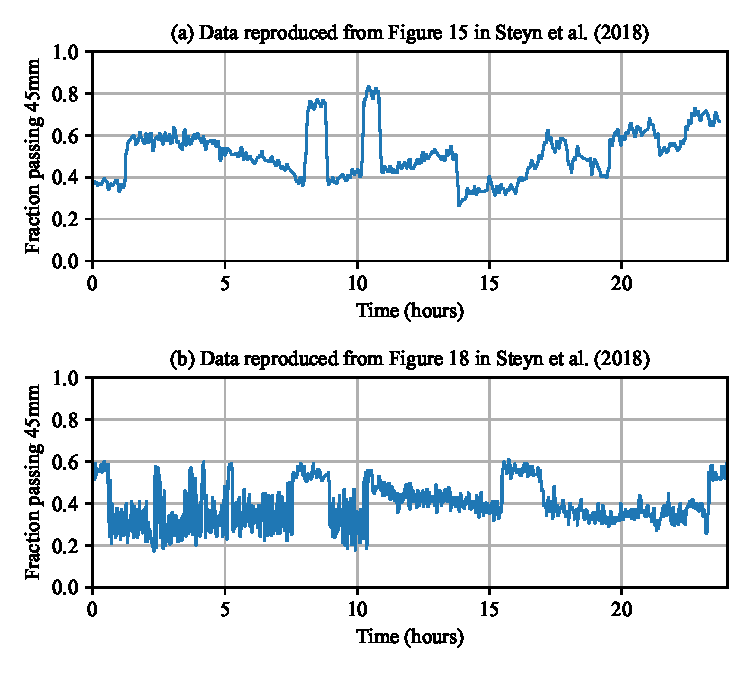
\includegraphics[width=13cm]{images/tsdata-steyn-figs.pdf}
	\caption{Samples from online particle size analysers}
	\label{fig:ind-data-tsplots}
\end{figure}

Recent innovations in ore hardness testing methods and equipment are starting to shed light on the nature of ore hardness variations in real operations. However, current methods still involve manual sampling and testing activities, which limits the frequency of measurements and makes them cost-prohibitive for ongoing monitoring \citep{kojovic_value_2019}.


\section{Objectives of the research} \label{sec:objectives}

From the literature review described in Section \ref{sec:lit-grinding}, it was apparent that changes in ore properties in the feed to the grinding process have been a focus of research for many years. Many of the studies included step changes in particle size and hardness (or breakage rates) in control simulation experiments. There is evidence that ore feed disturbances have significant impacts on the grinding process and therefore pose a problem for process control, which aims to reduce variation in the main process variables. This problem is compounded by the fact that many of the internal states of the process are not measurable and models of the process dynamics have so far been found to be unobservable given the process measurements available in typical operations. 

Although some studies report the absolute magnitude of variations in ore properties, there is a lack of publicly-available data on the dynamic nature of ore disturbances. What data there are (see \cite{steyn_investigating_2018} for example), suggest that this dynamic behaviour is complex, including step changes, ramps and abrupt changes in the magnitude of high frequency variations. Based on the literature reviewed here, there has been no work on developing specialised disturbance models for grinding process control, or in incorporating such models into process observers to improve state estimation.

The objectives of this research are:
\begin{enumerate}
	\item Propose a model for representing disturbances in grinding process operations
	\item Propose an observer framework using this model.
\end{enumerate}
% More specific objective?
%This work aims to address the problem of detecting and estimating infrequent, abrupt changes in the ore feed.
A search of the academic literature was carried out to identify work on industrial process disturbances potentially relevant to grinding process control. The results of this are described in the next section.


\section{Literature review part 2 – disturbance models} \label{sec:lit-disturb-models}

Few examples of academic work on characterising and modelling realistic industrial disturbances were found in the literature. Most of the literature on `disturbance models' or `disturbance characterisation' deals with the design of standard stochastic disturbance models, for example \cite{muske_disturbance_2002}, and \cite{pannocchia_robust_2003}, or is focussed mainly on detection and diagnosis of faults (i.e. unexpected disturbances), \cite{thornhill_advances_2007}, for example. In fault or anomaly detection, models of the normal behaviour of the process are used to identify when an \textit{unmodelled} disturbance occurs. A typical fault detection algorithm does not have a model of the actual disturbance. Therefore, its execution is suspended once the disturbance occurs and until normal operation has resumed. In contrast, the goal of this work is to use disturbance models for state estimation in the presence of disturbances.

Notable exceptions are some works on disturbances in specific applications such as wind power generation, vehicle suspension systems, and ship movement control. For example, \cite{papaefthymiou_mcmc_2008} used a Markov-chain Monte Carlo (MCMC) method to simulate wind speed for realistic dynamic simulations of renewable energy generation systems. An interesting stochastic process model, known as the \gls{BRW}, was found in the literature on economic modelling \citep{nicolau_stationary_2002}. This is used to represent economic or financial variables that have upper and lower limits, such as interest rates. Industrial processes variables also commonly have a normal operating range with lower and upper limits that are not exceeded during normal operation.

A few research works are explicitly concerned with `realistic disturbances' (loosely defined) in continuous industrial processes. These are sometimes referred to as \textit{deterministic disturbances} to distinguish them from standard disturbance models based on stochastic (random) noise models. One type of model in this category, which has received considerable attention, is described in the next section.

\subsection{Randomly-occurring deterministic disturbances} \label{RODDs}

\cite{macgregor_duality_1984} introduced the concept of the \textit{\acrlong{RODD}} (\acrshort{RODD}). This is a family of stochastic processes useful for modelling deterministic disturbances commonly encountered in real industrial processes, including  infrequently-occurring step changes, exponential changes, and ramps with changing slope. Disturbances of these types might result, for example, from set point changes made by an operator or, relevant to this work, changes in the properties of material feeding a process. While these disturbances may be deterministic, the key issue is that they are not predictable by the control system. Therefore, representing them with a stochastic process driven by a random variable is a reasonable way to emulate the behaviour for the purposes of control system design.

The structural form of a \gls{RODD} model is an \gls{ARIMA} process fed by a special \textit{random shock} signal which has the value zero most of the time but occasionally, according to a defined probability, has a value sampled from a normal distribution. Depending on the choice of \gls{ARIMA} process model, this can be used to simulate different types of \gls{RODD}s which may act on a process. The details of the \gls{RODD} model are described in Section \ref{sec:RODD}.

MacGregor and coworkers also showed that the optimal control law derived for a process perturbed by a \gls{RODD} is no different than that which would be derived for a process subject to a standard stochastic noise.  This is due to the common \gls{ARIMA} structure of the models and the fact that the expected value (i.e. mean) of the random shock signal in the \gls{RODD} model is zero, as it is for a Gaussian noise. As a result, it is well-suited to process control design.

\subsection{Detection and estimation of RODDs} \label{detection_RODDs}

\cite{robertson_detection_1995} described how unmeasured \gls{RODD}s perturbing a system can be estimated online using a \textit{multiple-model} filtering approach. Traditional methods such as Kalman filters are unable to efficiently estimate \gls{RODD}s due to the inevitable trade-off that must be made between the ability to track the disturbance when it occurs and the sensitivity to noise at other times. Multiple-model approaches involve simultaneously maintaining multiple hypotheses about the possible sequence of past disturbances. Each hypothesis is modelled by a separate Kalman filter with different parameters and the resulting state estimates are combined to produce a best-estimate of the system states \citep{jaffer_estimation_1971, buxbaum_recursive_1969, tugnait_detection_1982}.
% Unnecessary:
%Since the sequence of past random shocks is not known, each filter's state estimate is calculated assuming a different hypothetical sequence of past shocks. The estimates of some filters are therefore better than those of others, depending on how closely the shock hypothesis sequences match the actual disturbance. The overall best estimate of the states is computed by calculating the conditional probabilities of each hypothesis given the available measurement data, and this estimate is updated recursively each sample period using Bayesian inference.

Due to practical limitations, approximate methods are needed to limit the number of hypotheses and thus the number of Kalman filters required. These are collectively referred to as \textit{sub-optimal} methods. \cite{robertson_detection_1995} proposed a sub-optimal estimator specifically designed for use with systems containing \gls{RODD}s. It utilizes a combination of three approximation techniques. The first is known as \textit{sequence fusion}, which involves merging hypotheses which are identical over a pre-determined \textit{fusion horizon}. The merging procedure is based on the \gls{GPB} algorithm \citep{buxbaum_recursive_1969, jaffer_estimation_1971, tugnait_detection_1982, gustafsson_estimation_1993}. Secondly, since the random shocks in a \gls{RODD} are infrequent, they assume that two shocks are unlikely to occur in close succession. Thirdly, they limit the total possible number of shocks over the fusion horizon. This combination of sub-optimal methods allows their algorithm to maintain a longer detection horizon without requiring as many filters as other methods. A long detection horizon is necessary in situations where it takes many sampling intervals to discriminate between two or more independent \gls{RODD}s.

Robertson and co. presented results of simulating this sub-optimal multiple-model observer on a 2-input, 2-output, non-linear dynamical system representing a continuous stirred-tank reactor (CSTR) process. They compared the estimates produced by the multiple-model observer with two single extended Kalman filters (\acrshort{EKF}) each with a different noise parameter. One of the \gls{EKF}s was very sensitive to the measurement noise and the other was slow to respond to the \gls{RODD} step disturbances, while the multiple-model observer performed better than either \gls{EKF} in the example simulations.

\cite{eriksson_classification_1996} highlighted the important differences between \textit{infrequent disturbances}, such as those produced by the \gls{RODD} model, and \textit{omnipresent} or persistent disturbances. They argued that the standard stochastic noise model used in traditional system identification methods is unlikely to capture the effects of infrequent disturbances, despite the significant effect they have on the process. As a solution, they proposed using a multiple-model observer to simultaneously estimate and distinguish between different types of load disturbances. As an example, they demonstrated how this can be used to determine if a disturbance is acting at the input or the output of a process, given a batch of measurement data collected under closed-loop conditions.

The method involves grouping the filters of two (or more) multiple-model observers into one combined multiple-model observer. Each `bank' of filters represents a set of hypotheses relating to one of the possible disturbance models. The combined observer is then simulated on the data (offline) and the decision on which disturbance type is present is made based on which group of filters the most likely hypothesis belongs to. They provided results from simulation and a laboratory experiment to show that the method distinguishes and estimates the correct disturbance in each case.

For the multiple-model observer, they used an adaptive sub-optimal approach known as the \gls{AFMM} algorithm by \cite{andersson_adaptive_1985}. The \gls{AFMM} algorithm employs a technique called \textit{sequence pruning} \citep{tugnait_detection_1982}, which is an alternative to the fixed-length \textit{sequence fusion} approach used by \cite{robertson_detection_1995} and \textit{hypothesis merging} techniques \citep{blom_interacting_1988}. Sequence pruning involves the online deletion of hypotheses that have a low probability given the current measurements. The deleted sequences are replaced by new sequences to represent only the possible branches of the most likely sequence at the next sample time. Thus, the total number of sequences and corresponding filters that need to be maintained remains constant. The \gls{AFMM} algorithm also includes a procedure for online estimation of the measurement noise covariance, using a forgetting factor to control the speed of adaptation of the estimate \citep{andersson_adaptive_1985}.

In both multiple-model observer approaches by \cite{eriksson_classification_1996} and \cite{robertson_detection_1995}, the process model and the magnitude and frequency of the actual disturbance are assumed to be known.

Robertson and Lee published a second paper a few years later \citep{robertson_method_1998}. In this paper they reference \cite{andersson_adaptive_1985} on the topic of multiple-model algorithms.  However, the approach and sub-optimal method used is very similar to that in their 1995 paper, except that a modification was made to the random shock variance parameter, which is applied at every update during the detection interval rather than only once. They also used slightly different terminology, dropping the term randomly-occurring deterministic disturbances in favour of \textit{infrequently-occurring abrupt disturbances}.

Simulation results using a different system were presented, a three-state non-linear model of a heptane to toluene aromatization process, along with sum-of-squared estimation errors, averaged over 50 different simulations, which makes it easier to compare the observer performance. The process was subjected to two independent RODD step disturbances of two process parameters (the reaction rate coefficient and a heat transfer coefficient). The results show that the sum of the squared errors of the parameter estimates was 35\% lower with the sub-optimal observer than with either a single \gls{EKF} or the standard \gls{GPB} algorithm. This was attributed to the fact that their observer has a horizon of 90 minutes (using 22 filters), whereas the standard \gls{GPB} algorithm has a horizon of only 2 minutes (using 16 filters), which is not enough to detect the shock occurrences.

\subsection{Disturbance modelling using hidden Markov models} \label{sec:lit-hmm}
\label{hidden_markov_models}

\cite{wong_disturbance_2007} proposed a more general framework for modelling realistic industrial disturbances which have both continuous and discrete (i.e. modal) dynamics. In this framework, mode transitions are described by a finite-state \textit{Markov chain}. The model generating the Markov chain is referred to as a \gls{HMM} because it has unknown parameters (transition probabilities) which must be inferred from available measurements. The combined system, including discrete and continuous dynamics is termed a \gls{MJLS} \citep{costa_discrete-time_2005}. The \gls{RODD} model is a special case of the \gls{MJLS}.

%and other methods assuming noise inputs described by a \textit{mixture-of-Gaussians} (MOG),%

The \gls{HMM} disturbance model can represent a much wider set of disturbances with complex switching behaviour, such as intermittent drifts, outliers, and white noise that is probabilistically interspersed with integrating white noise, which is an example of dual-regime behaviour. Although \gls{HMM}s and \gls{MJLS}s were not novel concepts at the time, the authors claim that their use for disturbance modelling was limited. For references on prior work on \gls{MJLS}s by the control community, they referred readers to \cite{costa_discrete-time_2005}.

Unlike \cite{robertson_detection_1995} and \cite{eriksson_classification_1996}, who focused on state estimation, Wong and Lee also consider methods to identify the disturbance model from measurement data. The plant and Markov model parameters are simultaneously estimated using \gls{MLE} methods, specifically, the \gls{EM} algorithm \citep{dempster_maximum_1977}.

For state estimation, Wong and Lee used a second-order generalized pseudo-Bayesian algorithm (\acrshort{GPB2}) \citep{bar-shalom_estimation_1993}. They presented two numerical examples, comparing the prediction errors of the \gls{GPB2} observer using the identified \gls{MJLS} model, averaged over 500 simulations, to those of the best observer with a stationary (i.e. non-switching) model, and to those of a \gls{GPB2} observer which uses the actual system model.  The results show that the prediction errors of the \gls{GPB2} observer with the identified model were only 6 or 7\% higher than those of the \gls{GPB2} observer with the true model, and both are significantly less than those of the stationary observer.

One important limitation of the \gls{HMM} approach, which the authors noted, is that it is difficult to determine whether a given \gls{MJLS} is identifiable from input-output data \citep{vidal_observability_2002}. For this reason, they chose examples which only have switching in the noise parameters. Another problem is that \gls{MLE} optimization is typically non-convex and the \gls{EM} algorithm will usually only find local optima. To achieve the results presented, Wong and Lee chose initial settings for the unknown parameters that were known to be close to the global solution.

\cite{wong_realistic_2009} built on the 2007 paper by demonstrating how the proposed \gls{HMM}-based disturbance framework can be integrated into existing model-based control formulations. After introducing the \gls{HMM} framework again, they presented three simulated process control examples. The first demonstrates the use of the \gls{HMM} disturbance framework for offset-free linear \gls{MPC} on a single-input, single-output system. Multiple simulation scenarios with different combinations of high or low noise at the inputs and outputs are tested and one with switching noise levels. The results show that the proposed \gls{MPC} designed with the \gls{HMM} model and \gls{GPB2} estimator yielded the best performance over all simulation scenarios, even when there is model-plant mismatch.

The second example demonstrates the closed-loop performance of the \gls{HMM} control strategy in detecting and rejecting deterministic step changes. The controller was compared to a well-tuned controller with an integrated white noise disturbance model.

In the third example, the \gls{HMM} framework was used to mitigate the impact of large variations in the concentration of the feed stream entering a non-linear ethanol fermentation process simulation model. The concentrations of the feed were modelled as switching infrequently among several mean levels (low, mid, and high) with the transitions governed by a Markov chain. In this example, a \textit{sequentially-linearized} \gls{MPC} \citep{lee_extended_1994} was used and the effects of different types of feedback were compared---full state feedback including the Markov decision variable, Markov decision variable and output feedback only, and output feedback only.

Due to the difficulties of \gls{MJLS} model identification mentioned above, they bypassed the issue in this paper by assuming that the system, noise, and Markov parameters were known. Nevertheless, the authors concluded that the benefits of an \gls{HMM}-based disturbance framework are ``most immediately'' gained by incorporating them within an existing control methodology such as \gls{MPC}. No further work on realistic industrial disturbances since \cite{wong_realistic_2009} could be found.

\subsection{Hybrid dynamical systems} \label{sec:lit-hybrid}

The \textit{hybrid dynamical system} is the most general definition, encompassing dynamical systems with both continuous and discrete states \citep{van_der_schaft_introduction_2000}. As well as \gls{HMM}-based models, it includes models with any type of switching behaviour, such as those governed by logic.

Many physical systems and processes exhibit discontinuous behaviour (i.e. non-smooth changes in states such as steps or ‘jumps’). Since they are ubiquitous in nature as well as in human-engineered systems, the topic has received considerable attention in recent decades \citep{sworder_boyd_1999, bemporad_identification_2001, costa_discrete-time_2005, camacho_model_2010, djemai_hybrid_2014, estrada_hybrid_2014, guo_moving_2013, botha_hybrid_2018, bemporad_fitting_2018, oliveira_iterative_2020, piga_estimation_2020}. Methods of modelling and estimating hybrid systems can be applied to industrial disturbances, of which there is a large variety, many exhibiting complex discontinuous behaviour.

\subsection{Non-linear system identification}

Since the types of disturbance models of interest in industrial process control are non-linear, or utilise non-Gaussian probability density functions, standard linear system identification techniques are not applicable. The literature on non-linear system identification is extensive and covers a wide variety of classes of non-linear systems \citep{schoukens_nonlinear_2019}. Indeed, the field extends beyond control engineering.

% TODO:
% Mention  signal processing, edge or step detection methods. Wavelets, TVR.

The central problem when a random variable input to a system is non-Gaussian, or when the system is non-linear, is that the posterior probability density distribution of the state and output variables may be non-Gaussian. In a discrete dynamical system, where the states are computed recursively over many time-steps, the analytical derivation of the posterior distribution at time $t$ becomes intractable, except in a few trivial cases.
%TODO: Do I need a reference here?

Therefore, most approaches to non-linear system identification tend to be numerical in nature and involve approximations of the true (unknown) probability distributions. The \gls{GMM} is one general technique for representing diverse probability distributions.
% TODO: Reference for above?
% Note relevant:
% The task is more difficult because there are innumerable possible non-linear model structures, whereas in linear system identification, there is a finite and usually moderate number of model structures from which to choose.

%TODO:
%\begin{itemize}
%	\item Briefly explain the emergent use of numerical methods such as sequential Monte-Carlo for non-linear system identification \citep{schon_sequential_2015}, which includes particle filtering (Arulampalam, 2002 tutorial)
%	\item difference compared to \gls{MLE}/EM (\textit{Marginalization} vs. \textit{Data augmentation} – simultaneous state and parameter estimation) and (\text{frequentist} vs. \text{Bayesian} methods).
%	\item See overview diagram of methods in special issue of IEEE control magazine for an overview and cite this. \citep{wigren_nonlinear_2022}
%	\item Variational inference \citep{ma_multiple-model_2019}.
%\end{itemize}

\section{Contributions of the research} \label{sec:contributions}

The \gls{RODD} model was adopted for this work, due to its versatility and the fact that it can represent the specific types of disturbances of interest (infrequently-occurring step changes and ramp behaviour), as well as its simplicity, and the fact that it can be readily used in process control. It was not clear from the literature which of the multiple-model observers would be most suitable in grinding applications. Therefore it was decided to investigate both and attempt to resolve this question.

The main contributions of this work are:
\begin{enumerate}
	%\item Development of computer code to simulate two multiple-model observer algorithms for estimating \gls{RODD}s.
	\item Evaluation of the capabilities of two multiple-model observer algorithms for \gls{RODD} estimation by numerical simulation.
	\item Evaluation of the performance of the multiple-model observers applied to state estimation of a simulated grinding process with a switching ore feed disturbance.
	\item Comparison of the performance of the observers with a standard Kalman filter to identify advantages and disadvantages.
	%	\item Evaluation of the benefits of the multiple-model observer as part of a simulated control system applied to a multivariable grinding process with an ore feed disturbance.
	%\item \textbf{T.b.d.: A case study of the application of a disturbance model identification technique to characterise disturbances using simulated disturbance data and data from a real industrial operation.}
\end{enumerate}

The next chapter describes the methods in more detail.


